\documentclass[]{article}
\usepackage{graphicx}
\usepackage[svgnames]{xcolor} 
\usepackage{fancyhdr}
\usepackage{tocloft}
\usepackage[hidelinks]{hyperref}
\usepackage{enumitem}
\usepackage[many]{tcolorbox}
\usepackage{listings }
%\usepackage[a4paper, total={6in, 8in} , top = 2cm,bottom = 4cm]{geometry}
\usepackage[a4paper, total={6in, 8in} , top = 2cm,bottom = 4cm]{geometry}
\usepackage{afterpage}
\usepackage{amssymb}
\usepackage{pdflscape}
\usepackage{textcomp}
\usepackage{xecolor}
\usepackage{rotating}
\usepackage[Kashida]{xepersian}
\usepackage[T1]{fontenc}
\usepackage{tikz}
\usepackage[utf8]{inputenc}
\usepackage{PTSerif} 
\usepackage{seqsplit}
\usepackage{changepage}


\usepackage{listings}
\usepackage{xcolor}
\usepackage{sectsty}

\setcounter{secnumdepth}{0}
 
\definecolor{codegreen}{rgb}{0,0.6,0}
\definecolor{codegray}{rgb}{0.5,0.5,0.5}
\definecolor{codepurple}{rgb}{0.58,0,0.82}
\definecolor{backcolour}{rgb}{0.95,0.95,0.92}
\definecolor{blanchedalmond}{rgb}{1.0, 0.92, 0.8}
\definecolor{brilliantlavender}{rgb}{0.96, 0.73, 1.0}
 
\NewDocumentCommand{\codeword}{v}{
\texttt{\textcolor{blue}{#1}}
}
\lstset{language=java,keywordstyle={\bfseries \color{blue}}}

\lstdefinestyle{mystyle}{
    backgroundcolor=\color{backcolour},   
    commentstyle=\color{codegreen},
    keywordstyle=\color{magenta},
    numberstyle=\tiny\color{codegray},
    stringstyle=\color{codepurple},
    basicstyle=\ttfamily\normalsize,
    breakatwhitespace=false,         
    breaklines=true,                 
    captionpos=b,                    
    keepspaces=true,                 
    numbers=left,                    
    numbersep=5pt,                  
    showspaces=false,                
    showstringspaces=false,
    showtabs=false,                  
    tabsize=2
}

\lstset{style=mystyle}

 \settextfont[BoldFont={XB Zar bold.ttf}]{XB Zar.ttf}


\setlatintextfont[Scale=1.0,
 BoldFont={LiberationSerif-Bold.ttf}, 
 ItalicFont={LiberationSerif-Italic.ttf}]{LiberationSerif-Regular.ttf}





\newcommand{\inputsample}[1]{
    ~\\
    \textbf{ورودی نمونه}
    ~\\
    \begin{tcolorbox}[breakable,boxrule=0pt]
        \begin{latin}
            \large{
                #1
            }
        \end{latin}
    \end{tcolorbox}
}

\newcommand{\outputsample}[1]{
    ~\\
    \textbf{خروجی نمونه}

    \begin{tcolorbox}[breakable,boxrule=0pt]
        \begin{latin}
            \large{
                #1
            }
        \end{latin}
    \end{tcolorbox}
}

\newtcolorbox{mybox}[2][]{colback=red!5!white,
colframe=red!75!black,fonttitle=\bfseries,
colbacktitle=red!85!black,enhanced,
attach boxed title to top center={yshift=-2mm},
title=#2,#1}

\newenvironment{changemargin}[2]{%
\begin{list}{}{%
\setlength{\topsep}{0pt}%
\setlength{\leftmargin}{#1}%
\setlength{\rightmargin}{#2}%
\setlength{\listparindent}{\parindent}%
\setlength{\itemindent}{\parindent}%
\setlength{\parsep}{\parskip}%
}%
\item[]}{\end{list}}


\definecolor{foldercolor}{RGB}{124,166,198}
\definecolor{sectionColor}{HTML}{ff5e0e}
\definecolor{subsectionColor}{HTML}{008575}

\definecolor{listColor}{HTML}{00d3b9}

\definecolor{umlrelcolor}{HTML}{3c78d8}

\definecolor{subsubsectionColor}{HTML}{3c78d8}

\defpersianfont\authorFont[Scale=0.9]{XB Zar bold.ttf}


\defpersianfont\titr[Scale=1.5]{Lalezar-Regular.ttf}

\defpersianfont\fehrest[Scale=1.2]{Lalezar-Regular.ttf}

\defpersianfont\fehrestTitle[Scale=3.0]{Lalezar-Regular.ttf}

\defpersianfont\fehrestContent[Scale=1.2]{XB Zar bold.ttf}


\sectionfont{\color{sectionColor}}  % sets colour of sections
\subsectionfont{\color{subsectionColor}}  % sets colour of sections
\subsubsectionfont{\color{subsubsectionColor}}


\renewcommand{\labelitemii}{$\circ$}


\renewcommand{\baselinestretch}{1.1}


\renewcommand{\contentsname}{فهرست}

\renewcommand{\cfttoctitlefont}{\fehrestTitle}


\renewcommand\cftsecfont{\color{sectionColor}\fehrestContent\selectfont}
\renewcommand\cftsubsecfont{\color{subsectionColor}\fehrestContent\selectfont}
\renewcommand\cftsubsubsecfont{\color{subsubsectionColor}\fehrestContent\selectfont}
%\renewcommand{\cftsecpagefont}{\color{sectionColor}}

\setlength{\parskip}{1.2pt}

\begin{document}


%%% title pages
\begin{titlepage}
\begin{center}

\textbf{ \Huge{به نام خدا} }
        
\vspace{0.2cm}


\includegraphics[width=0.4\textwidth]{sharif1.png}\\
\vspace{0.2cm}
\textbf{ \Huge{\emph درس برنامه‌سازی پیشرفته} }\\
\vspace{0.25cm}
\textbf{ \Large{ فاز دوم پروژه} }
\vspace{0.2cm}
       
 
      \large \textbf{دانشکده مهندسی کامپیوتر}\\\vspace{0.1cm}
    \large   دانشگاه صنعتی شریف\\\vspace{0.2cm}
       \large   ﻧﯿﻢ سال دوم 99-98 \\\vspace{0.10cm}
      \noindent\rule[1ex]{\linewidth}{1pt}
اساتید:\\
    \textbf{{مهدی مصطفی‌زاده، ایمان عیسی‌زاده، امیر ملک‌زاده، علی چکاه}}



    \vspace{0.20cm}

   مهلت ارسال:\\
    \textbf{{27 خرداد - }}
    \textbf{{ساعت 23:59:59}}

    \vspace{0.10cm}
مسئول پروژه:\\
    \textbf{\authorFont{احمد سلیمی}}
    
        \vspace{0.10cm}
مسئولین فاز دوم:\\
    \textbf{\authorFont{سید مهدی فقیه و زﻫﺮا یوسفی جمارانی}}
    
        \vspace{0.10cm}
طراحان فاز دوم:\\
    \textbf{\authorFont{علیرضا تاجمیر ریاحی، سارا خسروی، آرمان زارعی، حمیدرضا کلباسی، ﮬﻤﻴﻠﺎ میلی }}
    
        \vspace{0.05cm}
مسئول تنظیم داک:\\
    \textbf{\authorFont{امیرمهدی نامجو}}
    

\end{center}
\end{titlepage}
%%% title pages


%%% header of pages
\newpage
\pagestyle{fancy}
\fancyhf{}
\fancyfoot{}
\cfoot{\thepage}
\lhead{فاز دوم}
\rhead{
\includegraphics[width=0.1\textwidth]{sharif.png}\\
دانشکده مهندسی کامپیوتر
}
\chead{پروژه برنامه‌سازی پیشرفته}
%%% header of pages
\renewcommand{\headrulewidth}{2pt}

\KashidaOff



\tableofcontents

\newpage

 \Large \textbf{\\
}



\section*{{\titr نکات قابل توجه}}
\addcontentsline{toc}{section}{{\fehrestContent نکات قابل توجه}}
\begin{itemize}
\item
پس از اتمام این فاز، در گیت خود یک تگ با عنوان \lr{"phase\_2"} بزنید. در روز تحویل حضوری این tag بررسی خواهد شد و کدهای پس از آن نمره‌ای نخواهد گرفت.

\item
در روز تحویل حضوری مشارکت تمام اعضای تیم در پروژه بررسی خواهد‌ شد و در صورت عدم مشارکت بعضی از اعضا، نمرهٔ ایشان برای آن فاز پروژه "صفر" لحاظ می‌گردد. مشارکت، با توجه به commit های افراد تیم در مخزن گیت‌هاب پروژه بررسی می‌شود.

\item
در هر فاز می‌توانید سه روز تاخیر به ازای کسر نمره داشته‌ باشید که به ازای هر روز آن، ۱۰ درصد از نمرهٔ آن فاز را از دست خواهید‌ داد. در مجموع سه‌فاز پروژه، سه روز تاخیر نیز بخشیده خواهد‌ شد.

\item
به ازای هر ساعتی که پروژه را زودتر تحویل دهید، ۱۵ دقیقه به مهلت تاخیر بدون کسر نمره شما اضافه خواهد‌ شد. این مقدار حداکثر یک روز خواهد‌ بود که در صورت ارسال ۴ روز زودتر از ددلاین به شما تعلق خواهد گرفت.

\item
در صورت کشف تقلب از هریک از تیم‌ها، برای بار اول منفی نمرهٔ آن فاز برای آن تیم ثبت می‌شود و برای بار دوم، نمرهٔ منفی کل پروژه برای تیم لحاظ خواهد‌ شد که معادل مردود شدن در درس است.
\end{itemize}

\newpage

\section*{{\titr توضیحات کلی}}
\addcontentsline{toc}{section}{{\fehrestContent توضیحات کلی}}

\textbf{\textcolor{red}{توجه بسیار مهم:}}
حتما داک نمرات این فاز را به دقت بررسی نمایید؛ پیاده سازی شما باید شامل آن موارد باشد تا نمره هر کدام را بگیرید. هرگونه پیاده‌سازی یا طراحی اضافه‌تر، کاملاً اختیاری، و فاقد نمره‌ی اضافه می‌باشد. در این داک فقط کلیت پیاده سازی ذکر شده است.

در این فاز شما باید گرافیکی برای لاجیک خود پیاده سازی کنید. توجه به نکات و راهنمایی‌های زیر شما را در پیاده سازی این فاز یاری می‌دهد:


\begin{itemize}
\item
نباید پیاده سازی لزوما به همان شکلی که در عکس‌ها می‌بینید انجام شود؛ ولی توجه کنید حتما باید بخش‌های الزامی را پیاده سازی کنید.

\item
عکس‌هایی که در قسمت‌های مختلف آورده شده است صرفا برای ایده گرفتن است و لزومی به پیاده سازی همانند آن نیست.


\item
\textcolor{red}{باید}
 از فونت‌های مناسب استفاده کنید؛ میتوانید از
   \href{https://www.kenney.nl/assets/kenney-fonts}{\textcolor{blue}{\underline{\lr{fonts}}}}
    و
     \href{https://www.behance.net/collection/4860923/Free-Fonts}{\textcolor{blue}{\underline{\lr{free-font }}}}
    استفاده کنید.

\item

می‌توانید از سایت‌های
 \href{https://www.flaticon.com/}{\textcolor{blue}{\underline{\lr{flaticon}}}} 
 - 
 \href{https://icons8.com/}{\textcolor{blue}{\underline{\lr{icons8}}}}
  -
   \href{https://www.iconninja.com/}{\textcolor{blue}{\underline{\lr{icon ninja}}}}
   آیکون‌های مورد نیاز خود را پیدا کنید.

\item

می‌توانید با استفاده از مستطیل و شفاف سازی آن‌ها مانند
 (\href{https://raw.githubusercontent.com/titansarus/Documents/master/phase_2/main/images/img1.jpg}{\textcolor{blue}{\underline{{این عکس}}}})  و یا با استفاده از عکس‌های مختلف  دکمه‌های مورد نیاز خود را بسازید. همچنین در 
  (
\href{https://hannemann.itch.io/ui-button-pack-free}{\textcolor{blue}{\underline{\lr{button-pack}}}}
 - \href{https://www.vecteezy.com/vector-art/116983-digital-game-button}{\textcolor{blue}{\underline{\lr{round-button}}}}
  -
  \href{https://www.clickminded.com/button-generator/}{\textcolor{blue}{\underline{\lr{button-factory}}}} -
   \href{https://pngtree.com/free-png-vectors/hexagon}{\textcolor{blue}{\underline{\lr{hexagon}}}}
   ) می‌توانید انواع دکمه‌ها را مشاهده کنید.


\item

می‌توانید برای کل قسمت‌ها یا برای هر قسمت متناسب با آن، عکسی به عنوان background قرار دهید (و یا رنگ background را تغییر دهید) البته این مورد به جز
\textcolor{red}{صفحهٔ اصلی}
  برای دیگر صفحات اجباری نیست و نمره اضافه‌ای نیز ندارد. لینک‌های مرتبط:

\href{https://pngtree.com/free-backgrounds}{\textcolor{blue}{\underline{\lr{background}}}} 
-
 \href{https://raw.githubusercontent.com/titansarus/Documents/master/phase_2/main/images/img2.jpg}{\textcolor{blue}{\underline{\lr{background 2 }}}}
 -
  \href{https://github.com/titansarus/Documents/blob/master/phase_2/main/images/img3.jpg}{\textcolor{blue}{\underline{\lr{sale-background }}}} 


\item

ممکن است این آیکون‌ها به شما کمک کنند:

\href{https://gamedeveloperstudio.itch.io/ui-icons}{\textcolor{blue}{\underline{\lr{icons}}}}
 -
\href{https://www.kenney.nl/assets/game-icons}{\textcolor{blue}{\underline{\lr{icons}}}}
   -
\href{https://www.kenney.nl/assets/ui-pack}{\textcolor{blue}{\underline{\lr{ui\_icons}}}}
     -
      \href{http://vecteezy.com/vector-art/112447-preloader-ui-progress}{\textcolor{blue}{\underline{\lr{progress-icon}}}}
       -
       \href{https://www.vecteezy.com/vector-art/144976-set-of-coupon-sale-vectors}{\textcolor{blue}{\underline{\lr{sale-icon}}}}
       -
        \href{https://www.iconninja.com/tag/offer-icon}{\textcolor{blue}{\underline{\lr{offer-icon}}}}
         - 
         \href{https://www.iconninja.com/tag/add-icon}{\textcolor{blue}{\underline{\lr{buy \& add}}}}

\item

در هر بخش اگر عمل مورد نظر موفق نبود، باید خطای مناسب را نمایش دهید؛ توجه کنید که باید این خطاها حتما به صورت گرافیکی نمایش داده شوند ولی اجباری برای اینکه به چه شکلی باشند وجود ندارد و می‌توانید از عکس یا text یا … استفاده کنید.

می توانید از عکس‌های زیر ایده بگیرید:

\begin{center}
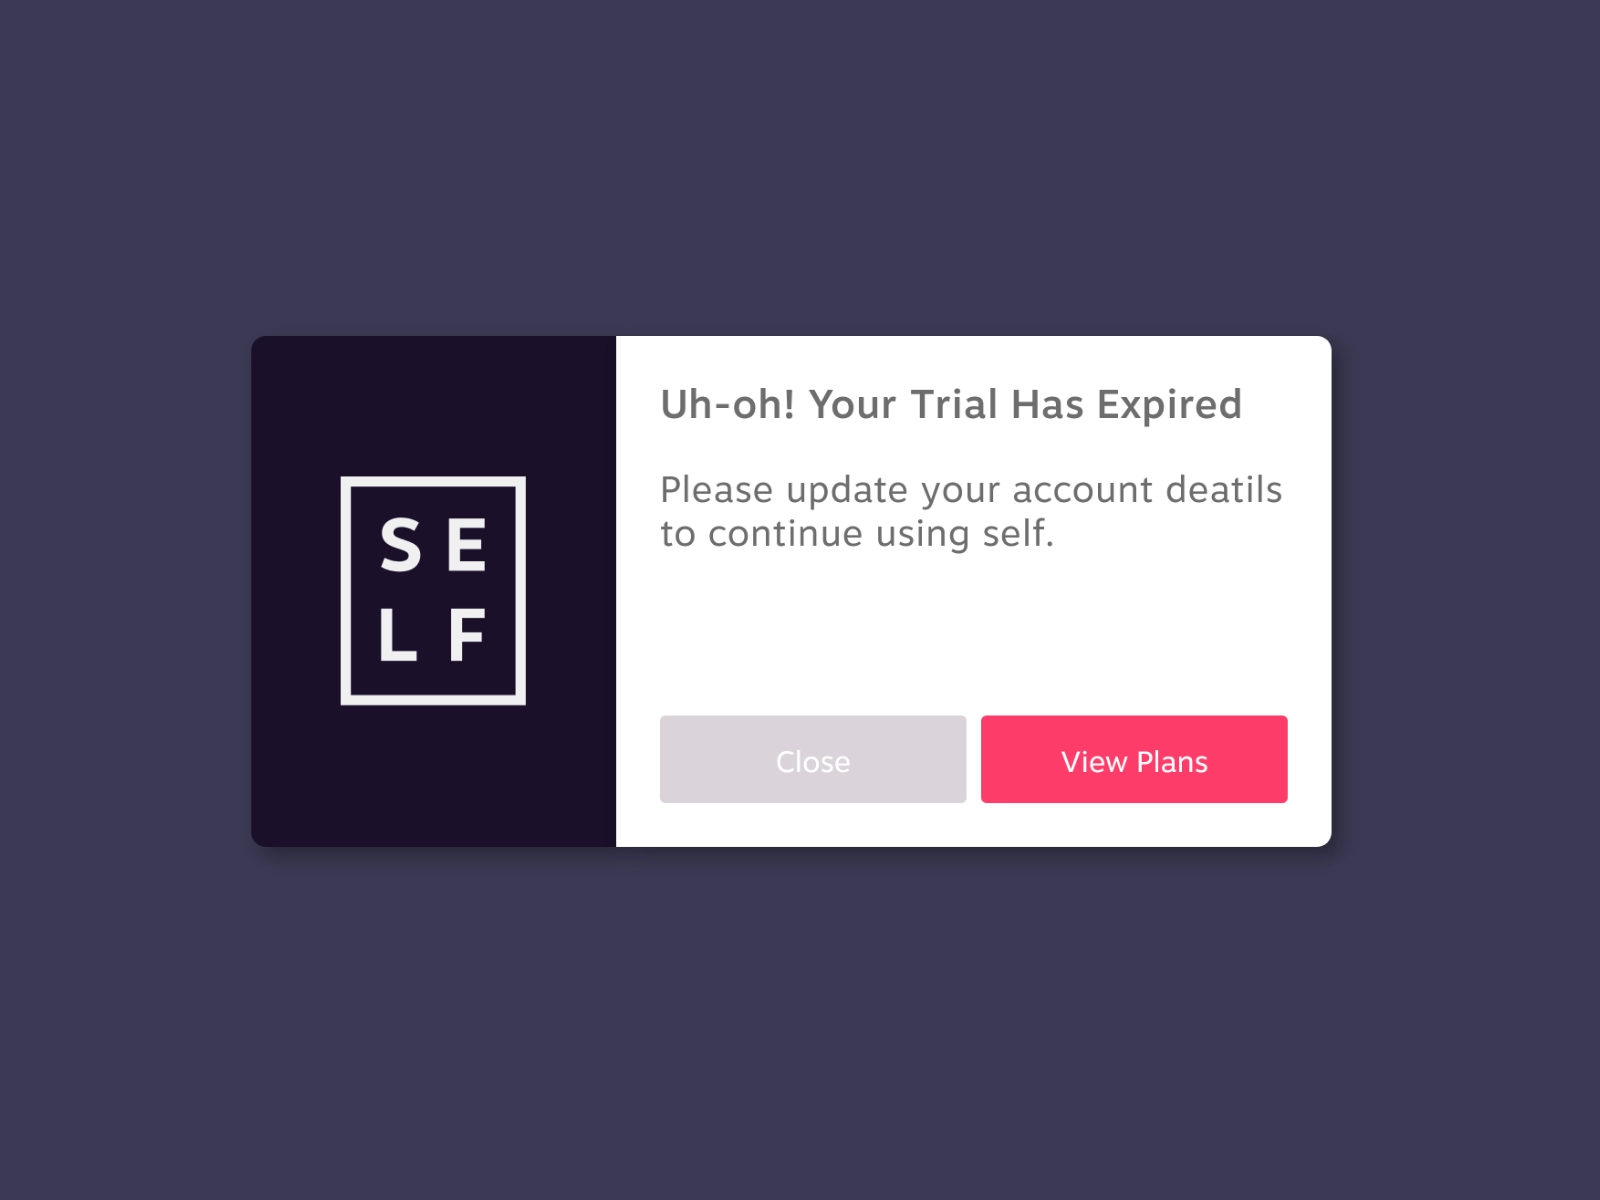
\includegraphics[width=0.7\textwidth]{images/image4.png}
\end{center}

\begin{center}
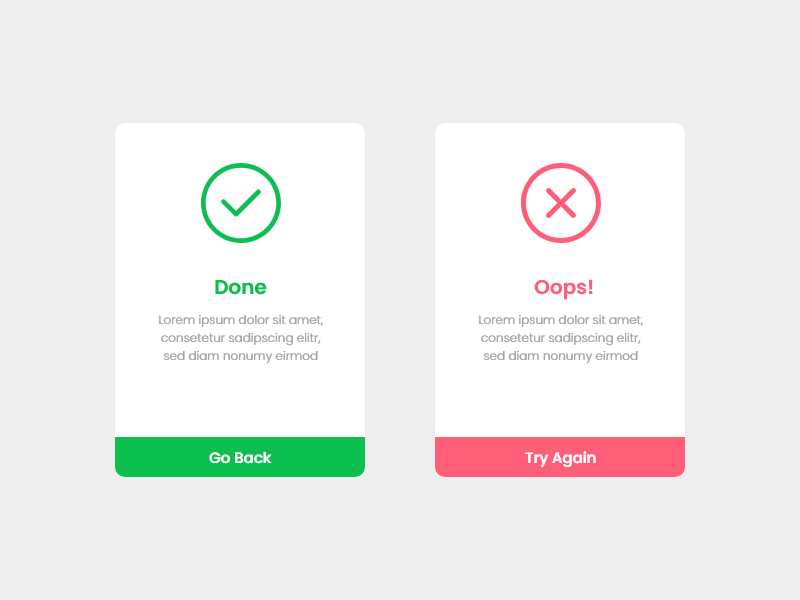
\includegraphics[width=0.7\textwidth]{images/image5.png}
\end{center}

\end{itemize}



\newpage

\section*{{\titr باید‌های پیاده‌سازی}}
\addcontentsline{toc}{section}{{\fehrestContent باید‌های پیاده‌سازی}}

\textbf{\textcolor{red}{توجه:}}
اگر زمانی که برنامه را اجرا می‌کنید، هنوز هیچ اکانت مدیری ساخته نشده است، باید ابتدا مشخصات اکانت مدیر دریافت شود و سپس وارد صفحهٔ اصلی برنامه شوید. در غیر این‌صورت(یعنی اگر مدیر وجود داشت) با اجرا کردن برنامه وارد صفحهٔ اصلی می شوید.

\subsection*{{\titr صفحهٔ اصلی}}

\addcontentsline{toc}{subsection}{{\fehrestContent صفحهٔ اصلی}}

شما باید یک منو برای انتخاب قسمت‌های مختلف یعنی ناحیه کاربری، محصولات و حراج‌ها داشته باشید.

\textbf{\textcolor{red}{توجه:}}
 دقت داشته باشید که برای این scene باید الزاما یکی از دو مورد زیر را نیز انجام دهید:

\begin{itemize}
\item
تغییر رنگ background

\item
قرار دادن عکسی به عنوان background

میتوانید از عکس‌های زیر ایده بگیرید:

\begin{center}

\includegraphics[width=0.3\textwidth]{images/image6.png}
\end{center}

\begin{center}
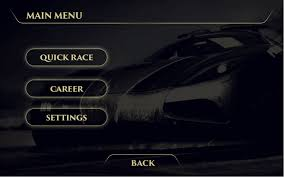
\includegraphics[width=0.6\textwidth]{images/image7.png}
\end{center}
\end{itemize}

\newpage

\subsection*{{\titr ناحیه کاربری}}
\addcontentsline{toc}{subsection}{{\fehrestContent ناحیه کاربری}}

 شما باید در این قسمت گرافیک تمام ناحیه کاربری که در فاز اول پیاده سازی کردید را پیاده سازی کنید.
 
اگر کاربر لاگین کرده باشد مشخصات و دسترسی‌های حساب کاربری نشان داده می‌شود؛ در غیر این صورت  امکان ثبت‌نام یا ورود برای کاربر وجود داشته باشد.

\textbf{\textcolor{red}{توجه:}}
 امکان دسترسی به ناحیه کاربری از تمام صفحات دیگر باید وجود داشته باشد.



\subsubsection*{{\titr پنل ثبت‌نام و ورود}}
\addcontentsline{toc}{subsubsection}{{\fehrestContent پنل ثبت‌نام و ورود}}

شما باید برای ثبت‌نام و همچنین ورود هر کاربر صفحه‌ای را پیاده سازی کنید. در صفحه‌ٔ‌ ثبت نام، باید برای دو نوع کاربر (خریدار و فروشنده)، فرم مربوط به آن موجود باشد و فیلدهای مربوط به هرکدام به کاربر نمایش داده‌ شود. توجه کنید که ثبت نام خریدار در صورت نبود مشکل بلافاصله انجام می‌پذیرد و بعد از آن می‌تواند login کند اما برای فروشنده، باید ابتدا ثبت نام آن توسط مدیر تایید شود و سپس می‌تواند login کند. پس از ورود نیز به همان صفحه‌ای که قبل از آن بوده می‌رود.


می‌توانید از عکس‌های زیر ایده بگیرید:






\begin{center}
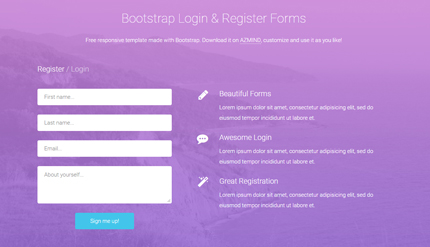
\includegraphics[width=0.9\textwidth]{images/image9.png}
\end{center}


\begin{center}
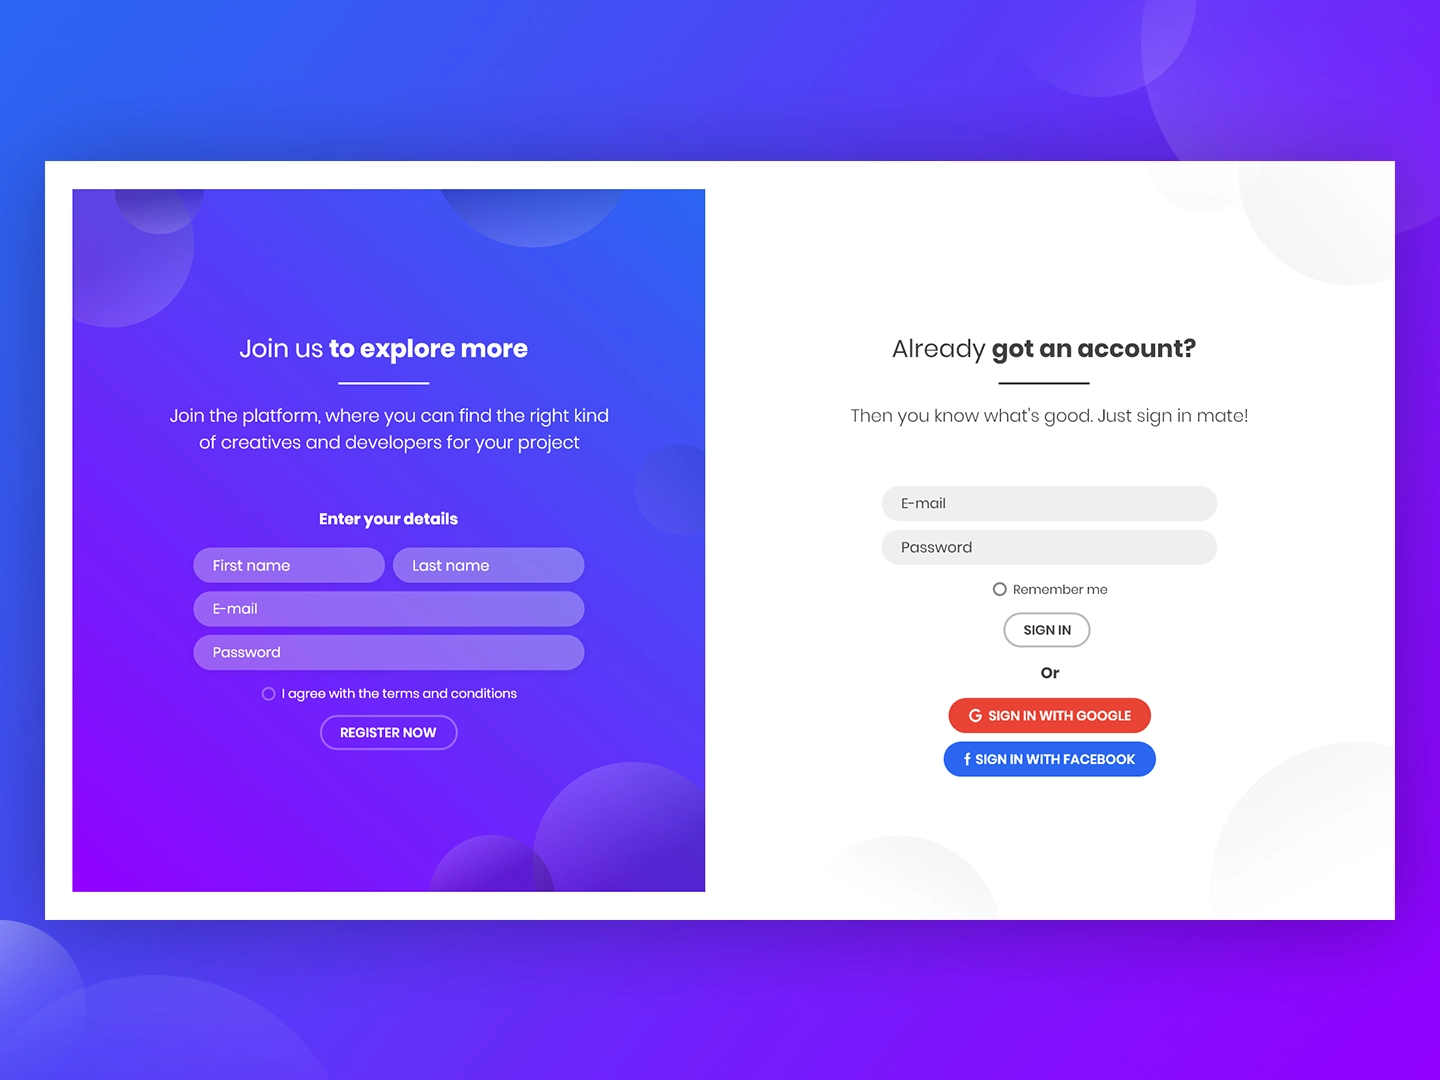
\includegraphics[width=0.9\textwidth]{images/image10.png}
\end{center}


\begin{center}
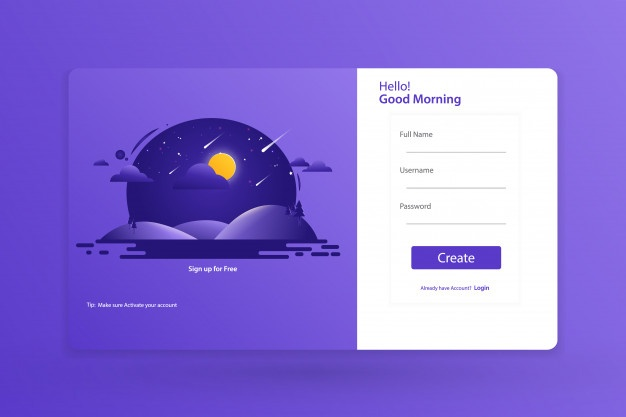
\includegraphics[width=0.9\textwidth]{images/image11.png}
\end{center}

\begin{center}
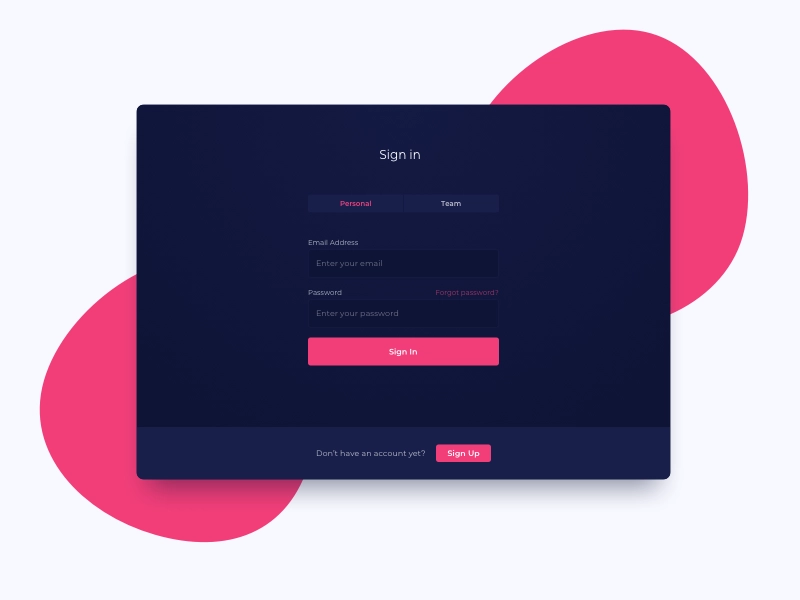
\includegraphics[width=0.6\textwidth]{images/image12.png}
\end{center}

\begin{center}
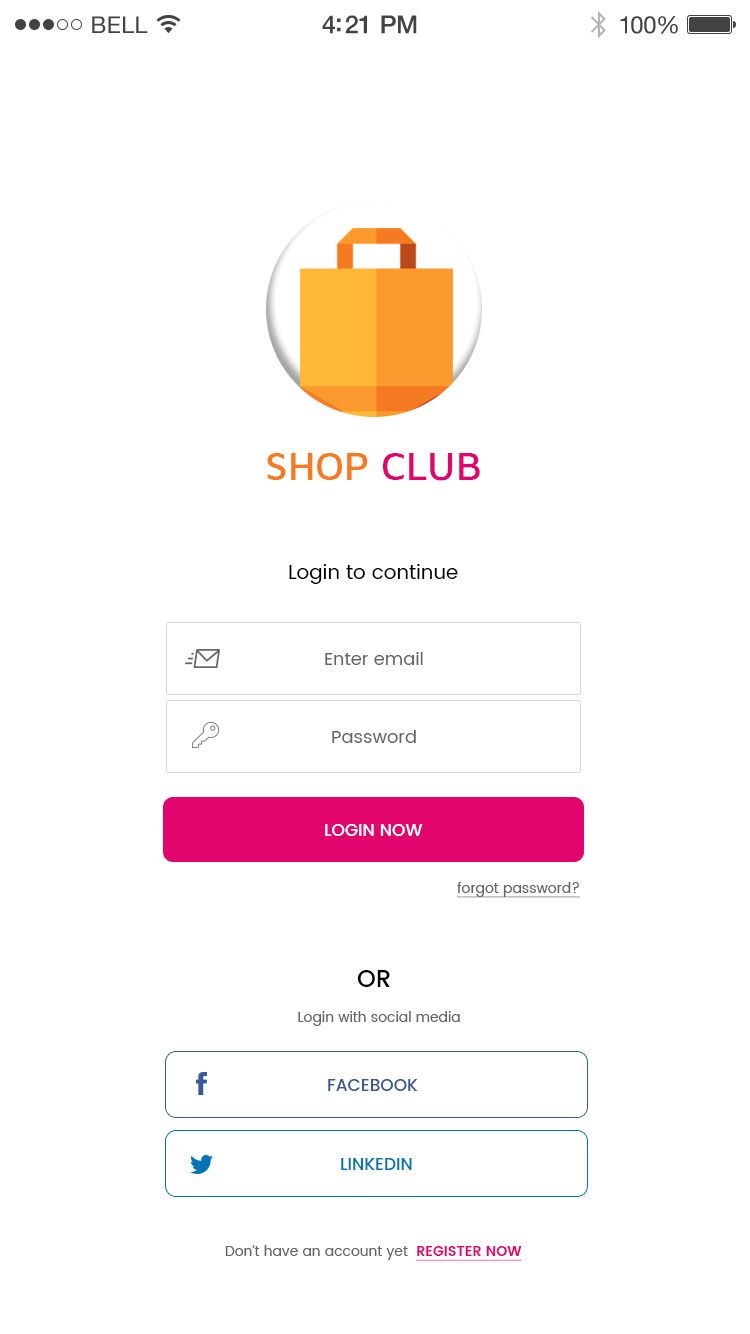
\includegraphics[width=0.6\textwidth]{images/image8.png}
\end{center}


\newpage


\subsubsection*{{\titr حساب کاربری}}
\addcontentsline{toc}{subsubsection}{{\fehrestContent حساب کاربری}}

شما باید صفحه‌ای برای نشان دادن اطلاعات کاربر داشته باشید؛ به عنوان مثال برای خریدار نمایش اطلاعات زیر الزامی است:

\begin{itemize}
\item
اطلاعات شخصی نظیر نام کاربری، نام، نام‌خانوادگی، ایمیل، شماره، رمز عبور

\item
نقش فرد (اگر فروشنده است اسم شرکت/کارگاه/کارخانه نیز ذکر شود.)

\item
دکمه انتقال به سبد خرید

\item
اعتبار

\item
دکمه‌ انتقال به صفحه سابقهٔ خرید

\item
لیست کدهای تخفیف شخص




\end{itemize}


برای مدیر و فروشنده نیز بایستی تمامی موارد گفته شده در فاز 1 را پیاده کنید.


می‌توانید از عکس‌های زیر ایده بگیرید:


\begin{center}
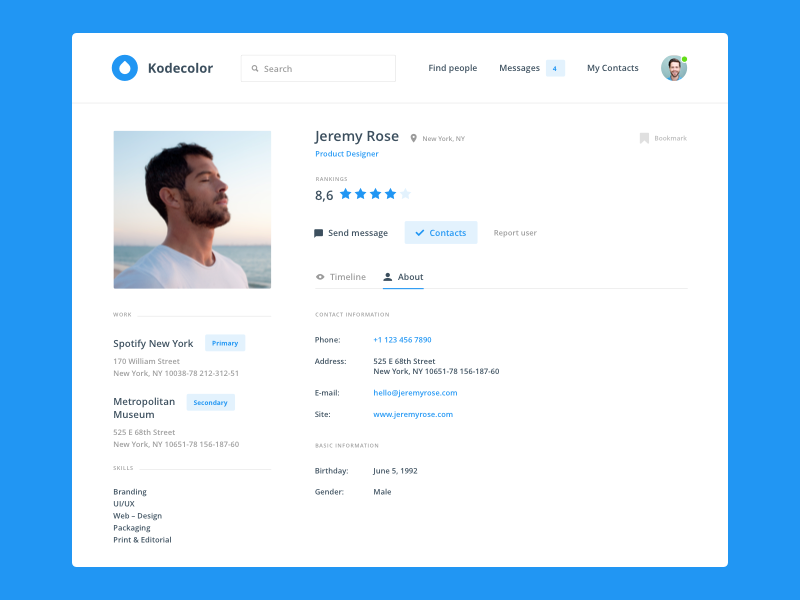
\includegraphics[width=0.9\textwidth]{images/image13.png}
\end{center}


\begin{center}
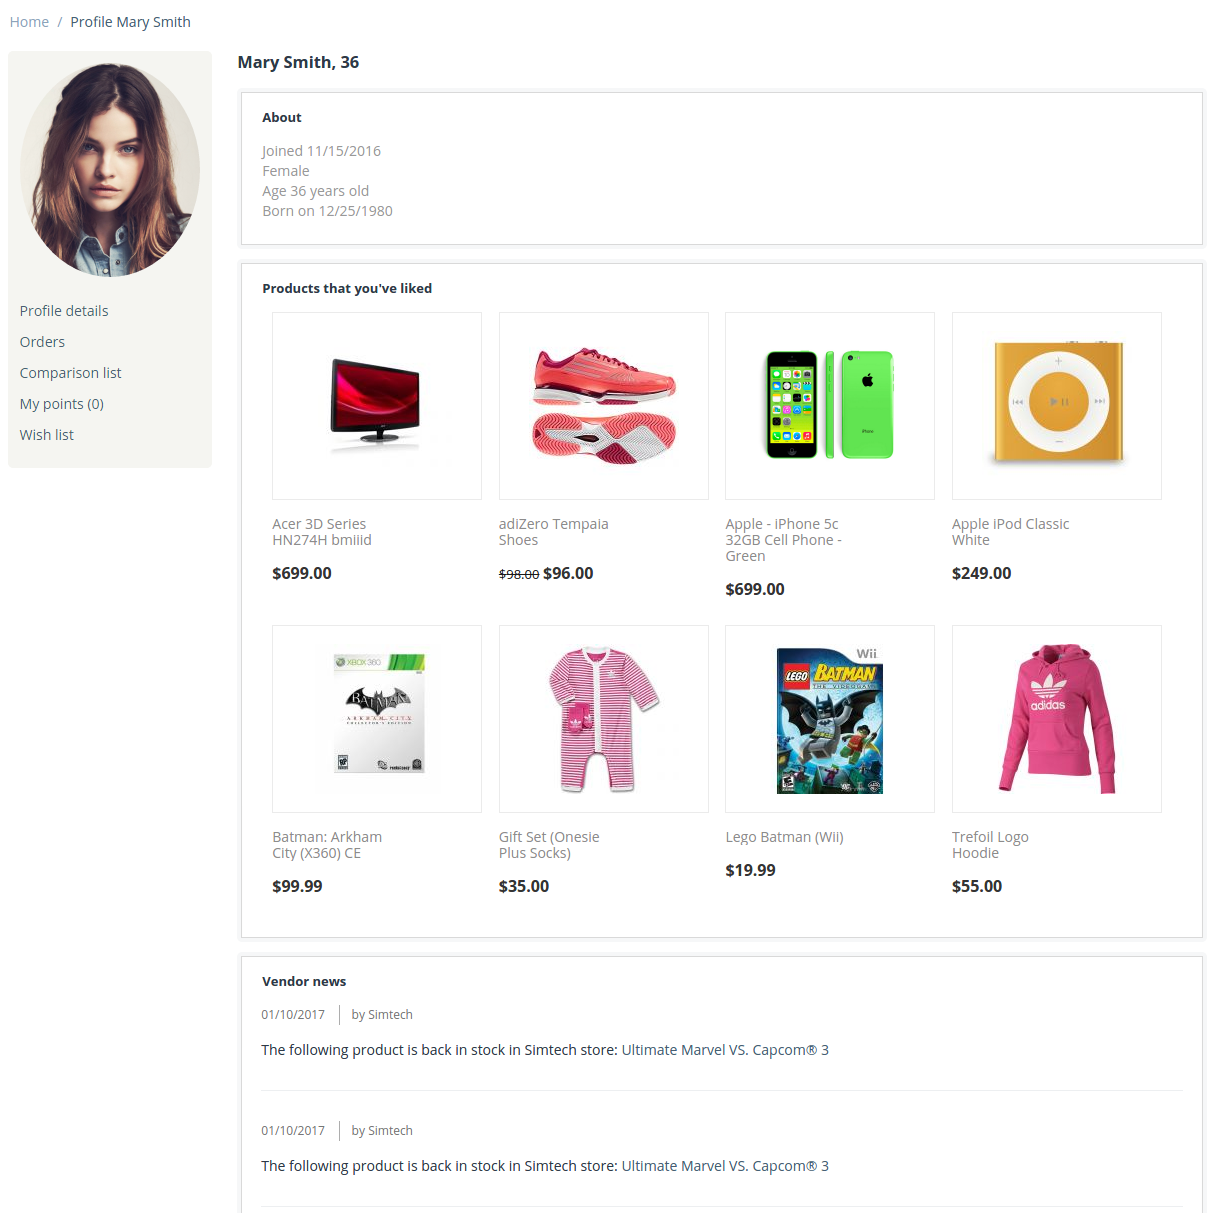
\includegraphics[width=0.9\textwidth]{images/image14.png}
\end{center}


\begin{center}
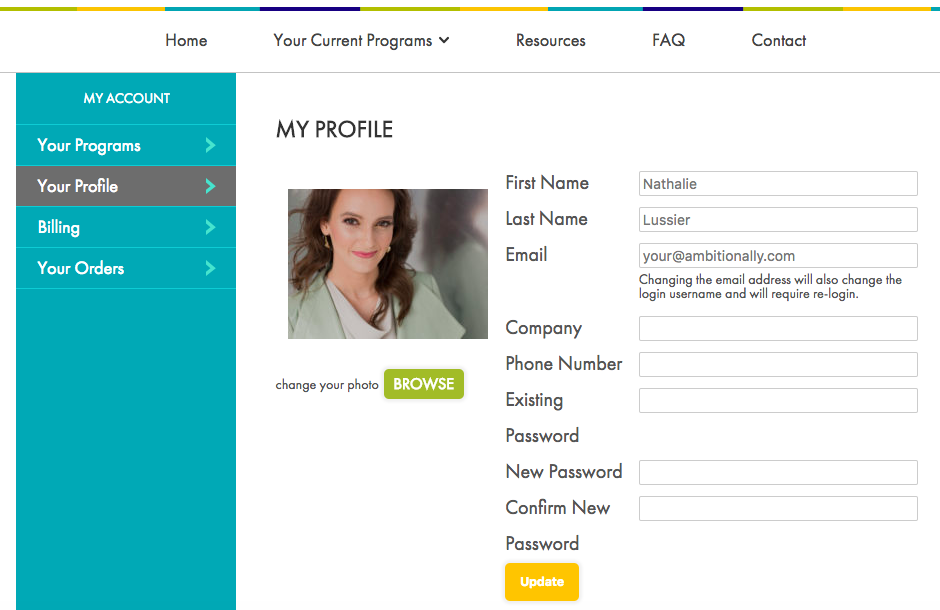
\includegraphics[width=0.9\textwidth]{images/image15.png}
\end{center}

\newpage

\subsection*{{\titr محصولات}}
\addcontentsline{toc}{subsection}{{\fehrestContent محصولات}}

\subsubsection*{{\titr صفحهٔ محصولات}}
\addcontentsline{toc}{subsubsection}{{\fehrestContent صفحهٔ محصولات}}


در این صفحه، باید لیست دسته‌بندی‌ها، ابزار sort، ابزار فیلتر و لیست محصولات طبق فیلتر اعمال شده و با ترتیبی که مشخص شده است نمایش داده شود. در حالت پیش‌فرض، هیچ فیلتری اعمال نشده است و همه‌ی محصولات به ترتیب تاریخ افزودن محصول نمایش داده می‌شوند.


\textbf{\textcolor{red}{توجه ۱:}}
برای اعمال فیلتر، کافیست یک دکمهٔ وجود داشته باشد که با زدن آن، لیست محصولات با توجه به فیلتر update شود.


\textbf{\textcolor{red}{توجه ۲:}}
 هر محصول در لیست محصولات باید دارای عکس، عنوان، قیمت و نمره باشد.


می‌توانید از عکس‌های زیر ایده بگیرید:


\begin{center}
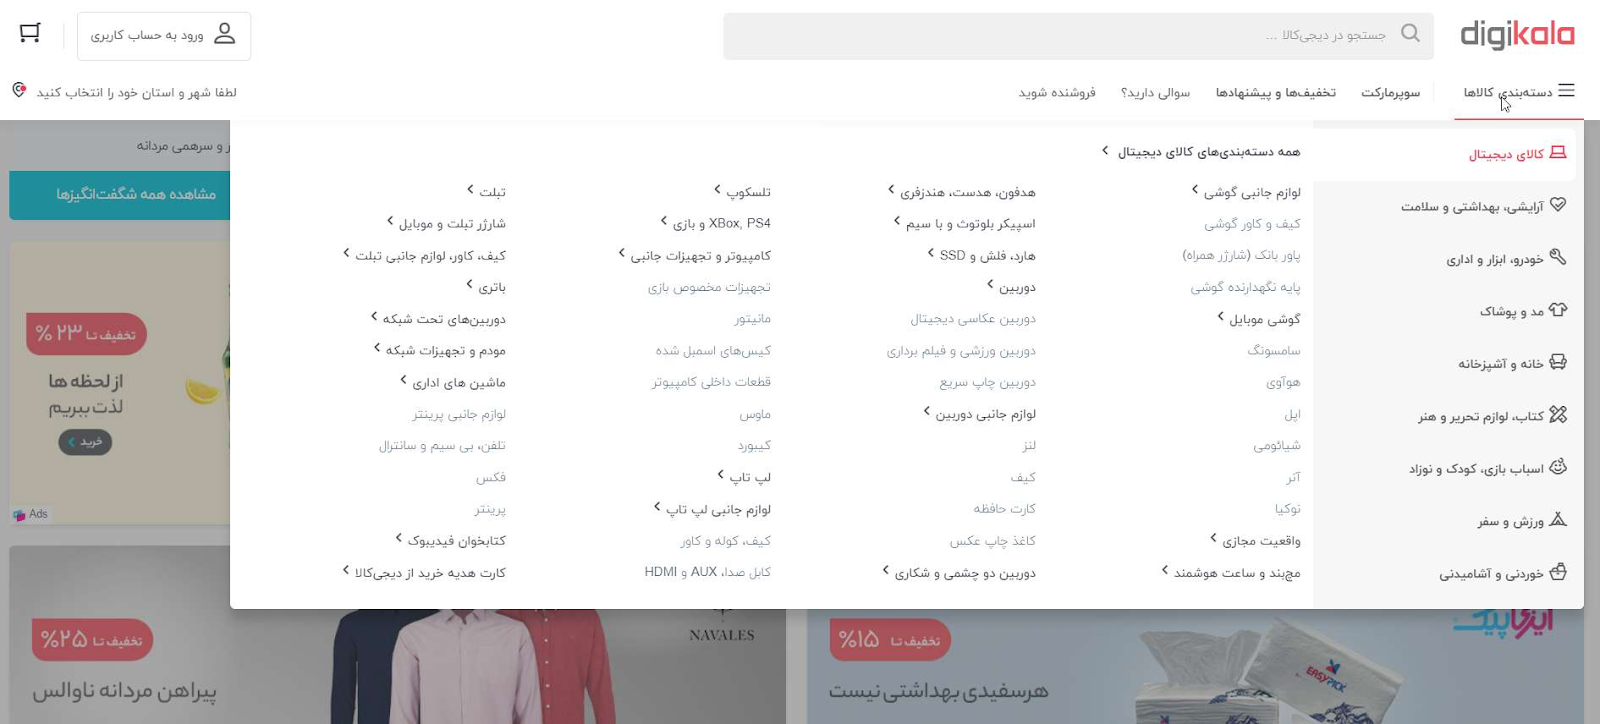
\includegraphics[width=0.9\textwidth]{images/image16.png}
\end{center}


\begin{center}
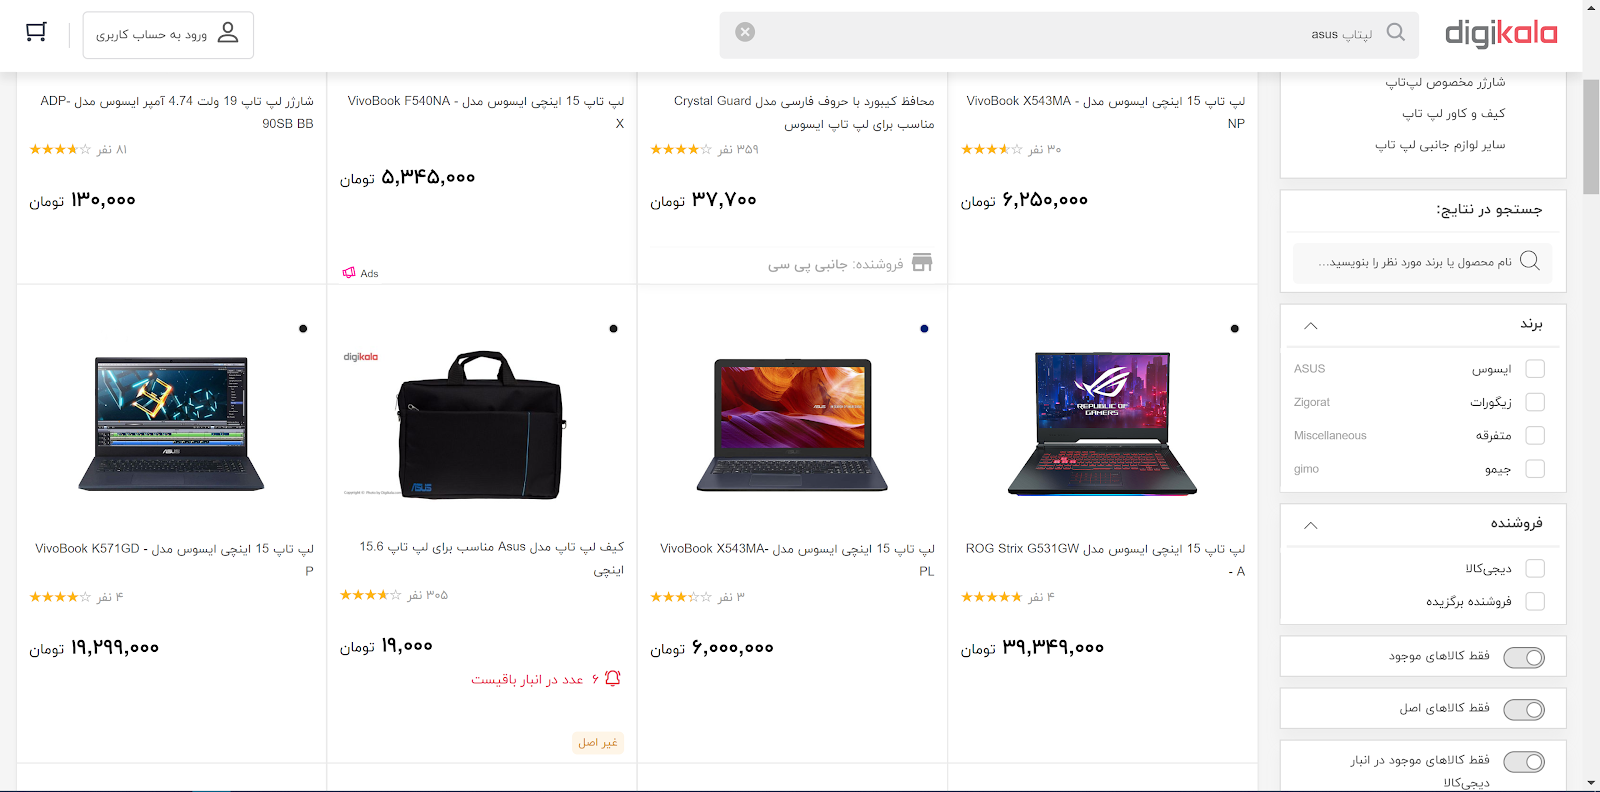
\includegraphics[width=0.9\textwidth]{images/image19.png}
\end{center}



\begin{center}
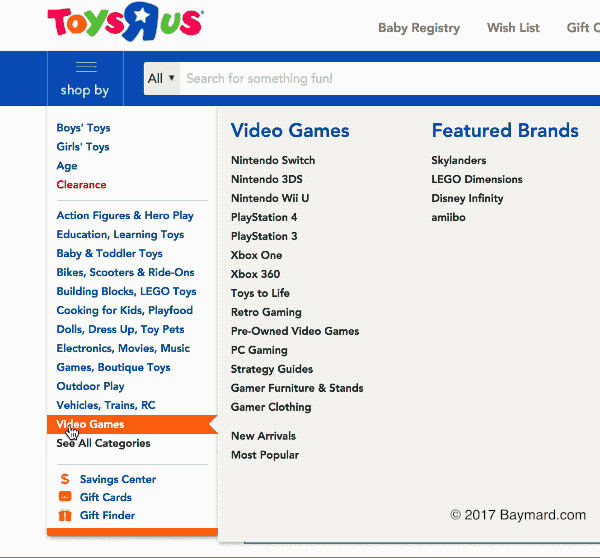
\includegraphics[width=0.7\textwidth]{images/image17.png}
\end{center}



\begin{center}
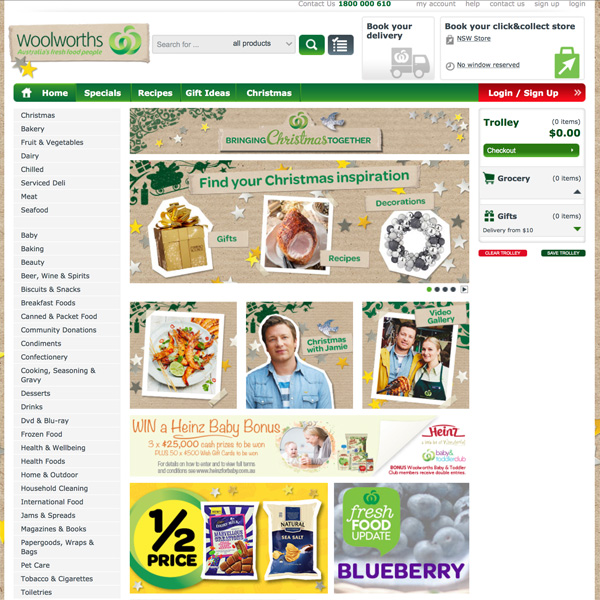
\includegraphics[width=0.7\textwidth]{images/image18.png}
\end{center}







\begin{center}
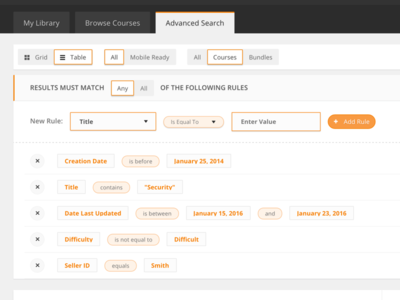
\includegraphics[width=0.9\textwidth]{images/image20.png}
\end{center}


\begin{center}
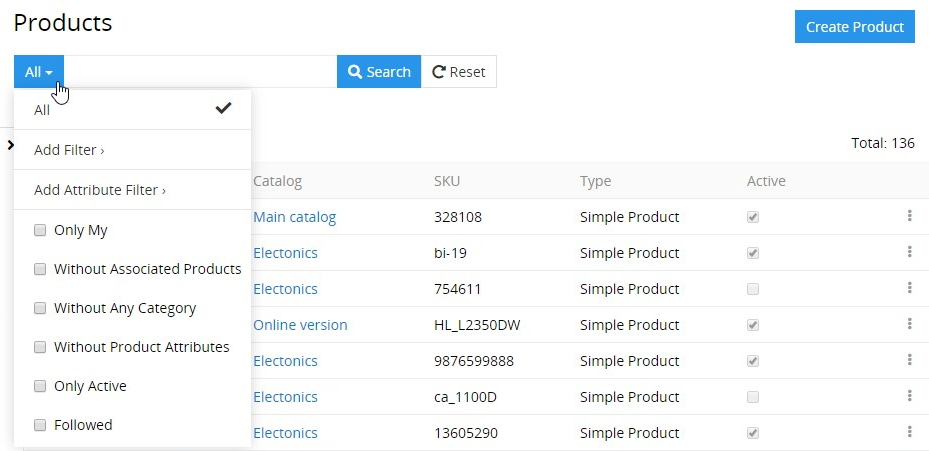
\includegraphics[width=0.9\textwidth]{images/image21.png}
\end{center}

\newpage
\subsubsection*{{\titr کالا}}
\addcontentsline{toc}{subsubsection}{{\fehrestContent کالا}}

باید صفحه‌ای داشته باشید که برای هر کالا هنگام کلیک بر روی آن، مشخصات آن کالا را نشان دهد. مواردی که باید حتما پیاده سازی شوند: 
\begin{itemize}
\item
ویژگی‌های عمومی (نام، توضیحات، قیمت، نمره و...) 

\item
ویژگی‌های خاص دسته‌بندی محصول

\item
 لیست نظرات (هر نظر شامل نام کاربری نظر دهنده، متن نظر و این که کالا را خریده یا نه است)
 
 \item
امکان نظر دادن

\item
نمره دادن به محصول (در صورتی که آن را خریده باشد)

\item 
دکمه‌ی افزودن به سبد خرید

\item
اگر از چند فروشنده پشتیبانی می‌کنید، لیست فروشندگان و قابلیت انتخاب فروشنده باید وجود داشته باشد.

\end{itemize}

می‌توانید از عکس‌های زیر ایده بگیرید:


\begin{center}
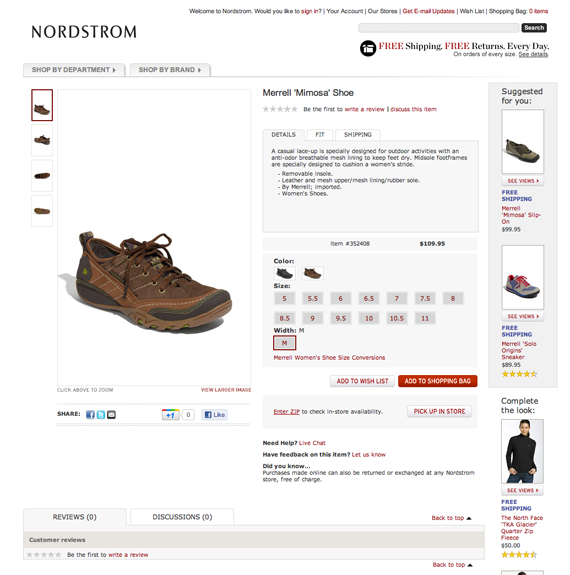
\includegraphics[width=0.7\textwidth]{images/image22.png}
\end{center}


\begin{center}
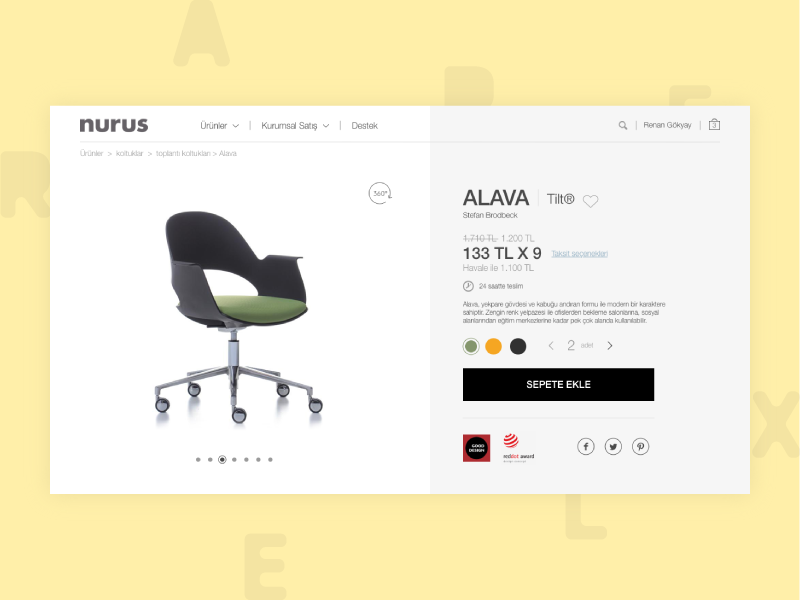
\includegraphics[width=1.0\textwidth]{images/image23.png}
\end{center}



\begin{center}
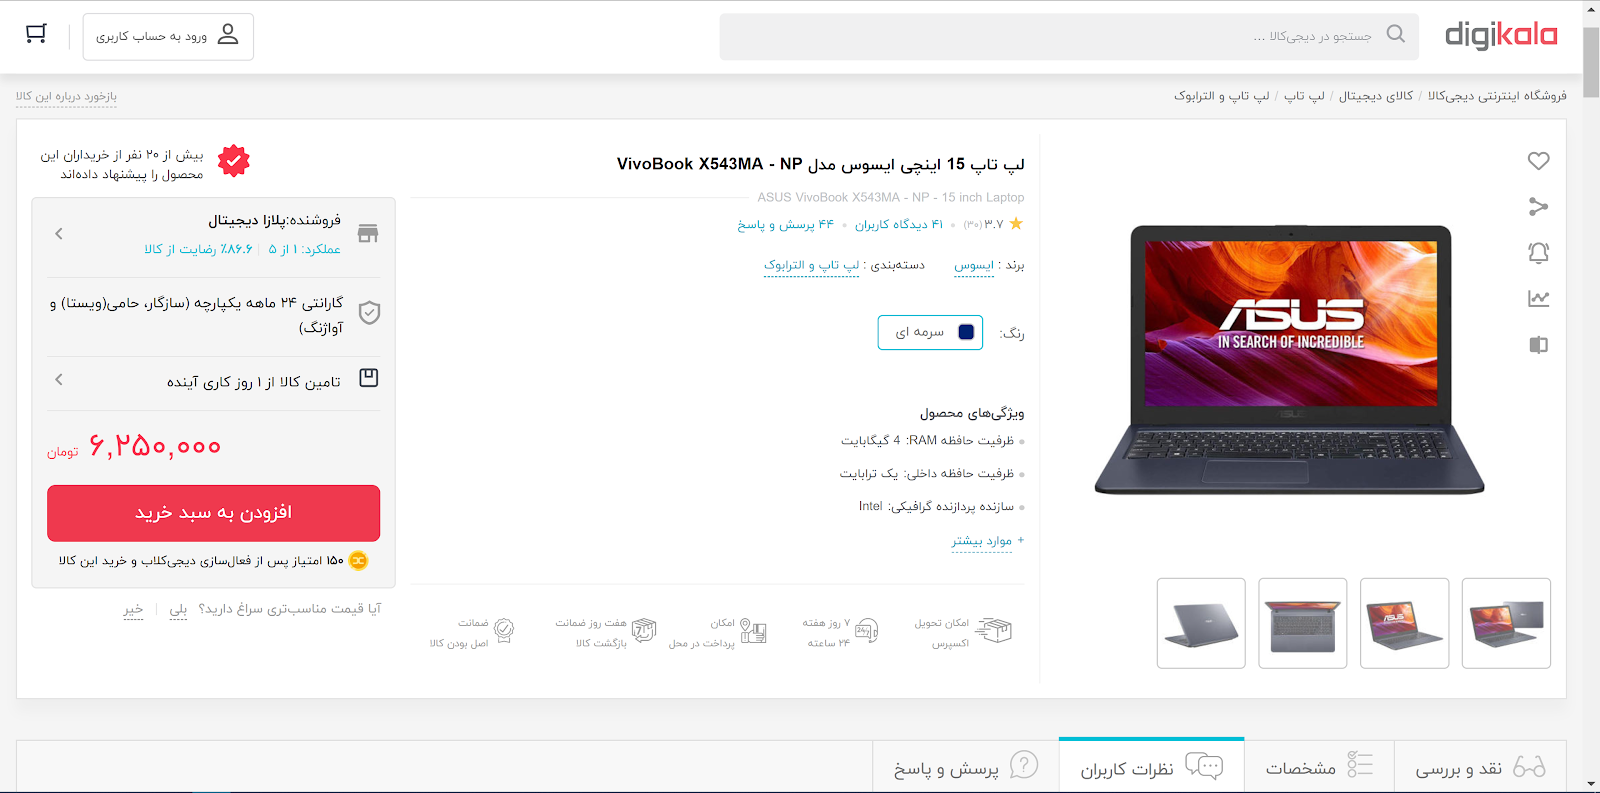
\includegraphics[width=1.0\textwidth]{images/image24.png}
\end{center}


\begin{center}
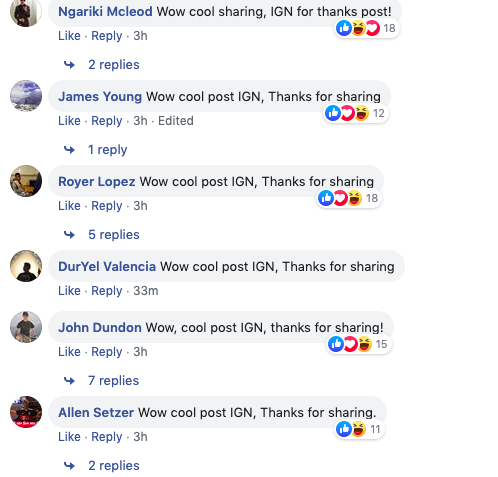
\includegraphics[width=0.9\textwidth]{images/image25.png}
\end{center}


\begin{center}
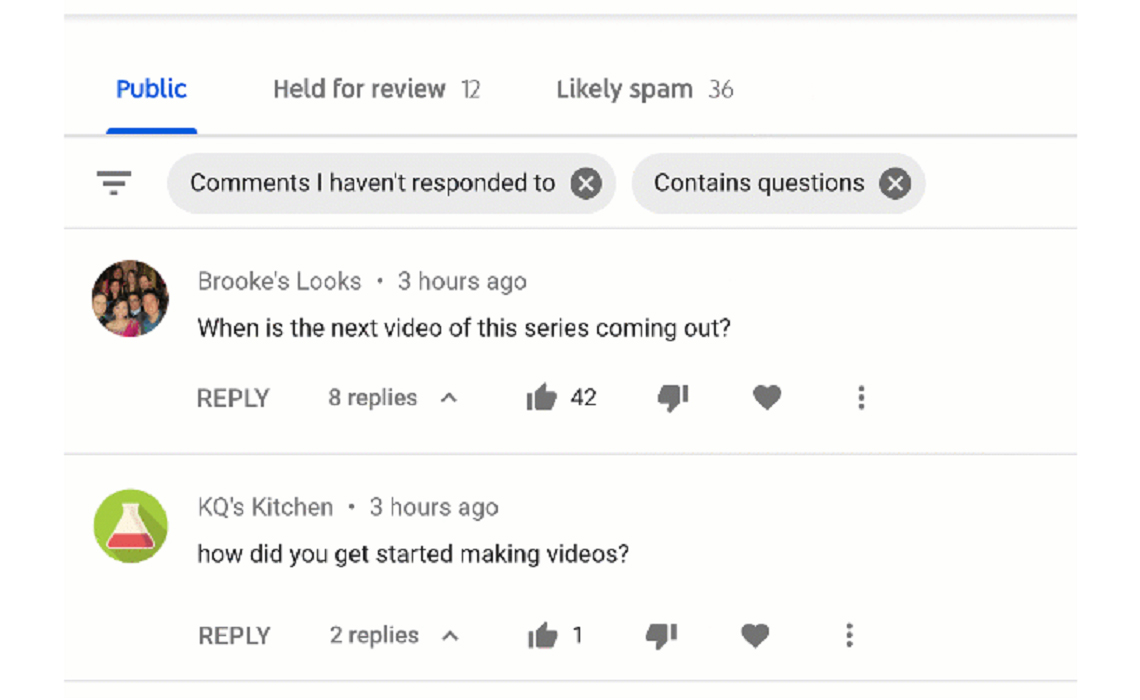
\includegraphics[width=0.9\textwidth]{images/image26.png}
\end{center}

\newpage

\subsection*{{\titr حراج‌ها}}
\addcontentsline{toc}{subsection}{{\fehrestContent حراج‌ها}}

شما باید صفحه‌ای برای نشان دادن حراج‌ها داشته باشید. ساختار این صفحه کاملا مشابه صفحهٔ محصولات است، با این تفاوت که فقط کالاهای دارای حراج را نمایش می‌دهد.

\textbf{\textcolor{red}{توجه ۱:}}
این صفحه را میتوانید به عنوان یک فیلتر (مثلا فیلتر تخفیف) در صفحه محصولات پیاده کنید. (در این صورت نیازی به داشتن دکمه ای برای انتقال به صفحهٔ حراج‌ها در منوی اصلی نیست)


\textbf{\textcolor{red}{توجه 2:}}
هر محصول در این لیست باید علاوه بر عکس، عنوان، قیمت و نمره،زمان باقی‌مانده به پایان حراج و میزان تخفیف را نیز شامل شود.


\subsection*{{\titr سبد خرید}}
\addcontentsline{toc}{subsection}{{\fehrestContent سبد خرید}}

شما باید صفحه‌ای برای نشان دادن سبد خرید کاربر داشته باشید. مواردی که باید حتما پیاده سازی شوند:

\begin{itemize}
\item
کالا‌های موجود در سبد خرید

\item
قیمت و تعداد کالاها

\item
هزینه نهایی اجناس موجود در سبد کالا

\item
گزینه‌ای برای افزایش یا کاهش تعداد کالای موجود در سبد کالا

\item
گزینه‌ای برای انتقال به صفحه پرداخت (در ادامه توضیح داده شده است)


\end{itemize}

\textbf{\textcolor{red}{توجه:}}
 در صورت کلیک بر روی هر محصول باید وارد صفحه مربوط به آن کالا شوید.
 
 
می‌توانید از عکس های زیر ایده بگیرید:


\begin{center}
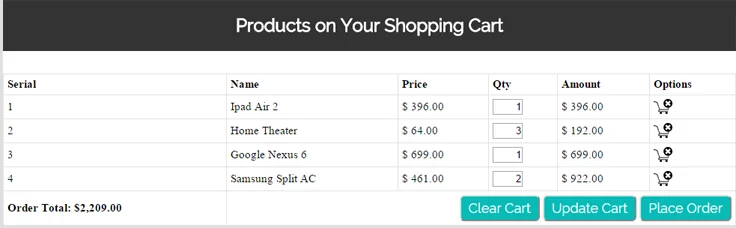
\includegraphics[width=0.9\textwidth]{images/image28.png}
\end{center}


\begin{center}
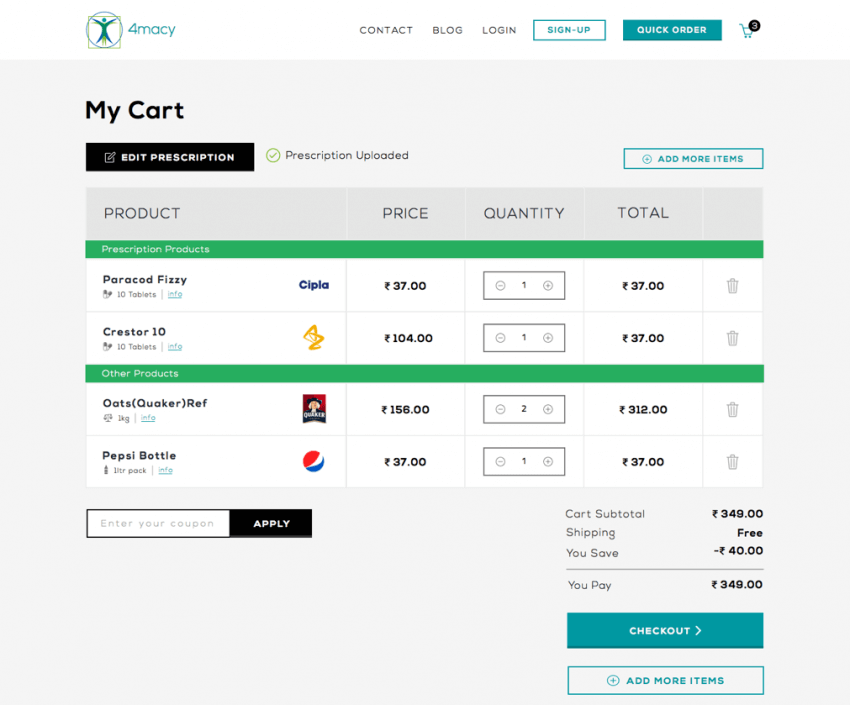
\includegraphics[width=1.1\textwidth]{images/image27.png}
\end{center}

\newpage


\subsection*{{\titr صفحه پرداخت }}
\addcontentsline{toc}{subsection}{{\fehrestContent صفحه پرداخت }}

در این صفحه باید مراحل زیر را به ترتیب پیاده کنید:

\begin{enumerate}
\item
اطلاعات دریافت‌کننده (آدرس، تلفن و...)

\item
دریافت کد تخفیف

\item
دکمهٔ پرداخت

\end{enumerate}

پس از زدن دکمهٔ پرداخت، گزارش نهایی خرید نمایش داده می‌شود. (اگر موفق بود تایید کسر مبلغ از اعتبار حساب، در غیر این صورت پیغام خطای مناسب نمایش داده شود.)

\textbf{\textcolor{red}{توجه:}}
 دقت کنید که مراحل بالا الزاما باید به ترتیب پیاده شوند و مثلا نباید وقتی که هنوز اطلاعات دریافت‌کننده وارد نشده است، دکمهٔ پرداخت نشان داده شود.


\subsection*{{\titr سابقهٔ خرید/فروش }}
\addcontentsline{toc}{subsection}{{\fehrestContent سابقهٔ خرید/فروش }}

در این صفحه بایستی لیست لاگ‌های خرید یا فروش کاربر را نمایش دهید و برای هر لاگ نیز تمام مشخصات آن -که در فاز 1 پیاده کردید- را نمایش دهید.

توجه کنید که می‌توانید این صفحه را با صفحه حساب کاربری ترکیب کنید ولی حتما بایستی این موارد پیاده شده باشند.


\newpage



\section*{{\titr ویژگی‌های انتخابی }}
\addcontentsline{toc}{section}{{\fehrestContent ویژگی‌های انتخابی }}

تمامی این موارد
\textbf{\textcolor{red}{نمره امتیازی}}
  دارند و اجباری برای پیاده سازی این موارد وجود ندارد:


\subsection*{{\titr صداگذاری }}
\addcontentsline{toc}{subsection}{{\fehrestContent صداگذاری }}


می‌توانید از آهنگی مناسب برای برنامه ی خود استفاده کنید؛ همچنین می توانید برای دکمه‌ها و ...
صداگذاری کنید.


در اینجا تعدادی سایت برای صداگذاری قرار داده‌ایم:

\href{https://www.kenney.nl/assets/impact-sounds}{\textcolor{blue}{\underline{\lr{sound}}}}
 -
  \href{https://www.kenney.nl/assets/digital-audio}{\textcolor{blue}{\underline{\lr{digital sound}}}}
   -
    \href{https://www.kenney.nl/assets/ui-audio}{\textcolor{blue}{\underline{\lr{ui sound}}}}
    -
     \href{https://www.zapsplat.com/}{\textcolor{blue}{\underline{\lr{sound-site}}}}


\subsection*{{\titr Animation Sprite  }}
\addcontentsline{toc}{subsection}{{\fehrestContent Animation Sprite }}

برای برخی از بخش‌ها می‌توانید از عکس‌های متحرک و یا Sprite ها استفاده کنید ( مثلا در بخش حراج، صفحه هر محصول و...)

\subsection*{{\titr بخش تبلیغات  }}
\addcontentsline{toc}{subsection}{{\fehrestContent بخش تبلیغات }}

می‌توانید در صفحه‌ی محصولات، بخشی برای نمایش تبلیغات داشته باشید؛ برای تبلیغ کردن یکی از کالاهای خود، در این قسمت باید به مدیر اصلی سایت درخواست دهید و در صورت تایید مدیر این تبلیغ میتواند نشان داده شود.

\textbf{\textcolor{red}{توجه ۱:}}
 یک کاربر فروشنده می‌تواند این درخواست را از طریق حساب کاربری به مدیر ارسال کند.

\textbf{\textcolor{red}{توجه 2:}}
هر فروشنده فقط یکی از محصولات خود را در آن واحد می تواند تبلیغ کند و در صورت تبلیغ محصولی دیگر، تبلیغ محصول قبلی لغو میشود. توجه کنید که برای هر تبلیغ، مقدار مشخصی از اعتبار فروشنده کسر می‌شود. همچنین هر تبلیغ یک ددلاین داشته باشد.

\newpage
\subsection*{{\titr up Pop  }}
\addcontentsline{toc}{subsection}{{\fehrestContent up Pop }}

می‌توانید مانند عکس زیر، در مواقع خاص همانند خرید ، حراج و ….. از این \lr{Pop up}  ها استفاده کنید؛ مثلا می‌توانید صفحه ورود را به صورت \lr{Pop up} پیاده کنید.



\begin{center}
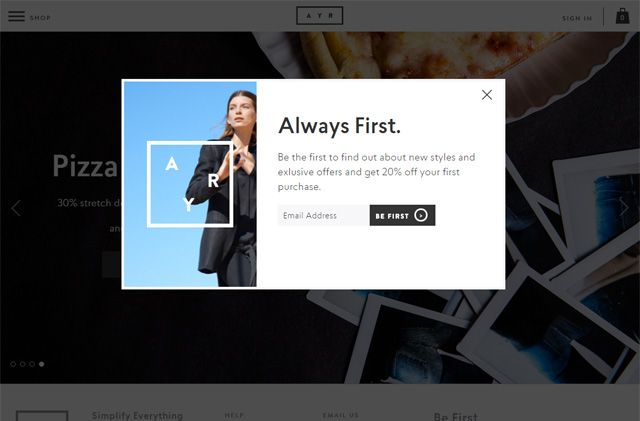
\includegraphics[width=0.9\textwidth]{images/image29.png}
\end{center}


\subsection*{{\titr امتیاز هر کالا   }}
\addcontentsline{toc}{subsection}{{\fehrestContent امتیاز هر کالا  }}

نمایش امتیاز کالا در صفحهٔ محصولات و صفحهٔ محصول، بصورت گرافیکی، مطابق عکس‌های زیر:


\begin{center}

\includegraphics[width=0.75\textwidth]{images/image31.png}
\end{center}

\begin{center}
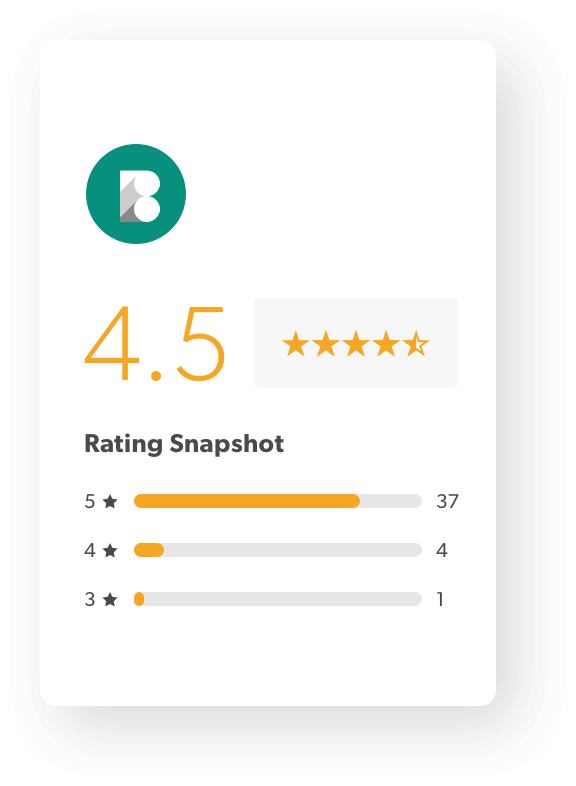
\includegraphics[width=0.6\textwidth]{images/image30.png}
\end{center}




\begin{center}

\includegraphics[width=0.8\textwidth]{images/image32.png}
\end{center}


\newpage


\subsection*{{\titr فیلتر Real-time   }}
\addcontentsline{toc}{subsection}{{\fehrestContent فیلتر real-time  }}

در این قسمت باید ابزار فیلتر را به گونه‌ای پیاده سازی کنید که با تغییر هر پارامتر فیلتر، لیست کالاها update شود. (بدون نیاز به دکمهٔ اعمال فیلتر)


\subsection*{{\titr Zoom   }}
\addcontentsline{toc}{subsection}{{\fehrestContent Zoom  }}

 با حرکت موس بر روی تصویر محصول نمای بزرگتری از محصول نمایش داده شود.
 
 
 
 \begin{center}
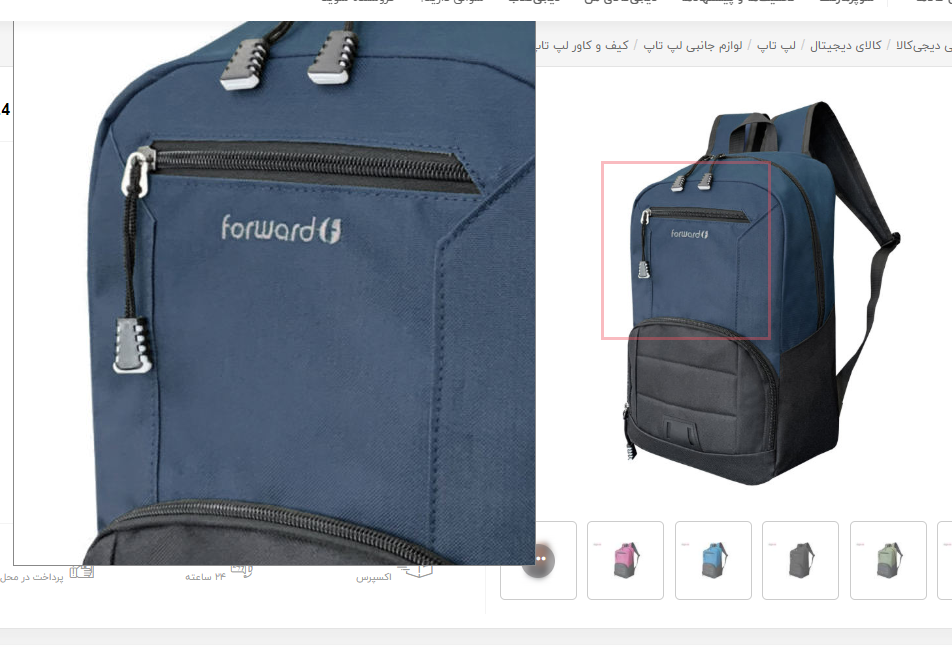
\includegraphics[width=0.9\textwidth]{images/image33.png}
\end{center}
 
 
 
\subsection*{{\titr تغییر عکس کالا متناسب وضعیت آن   }}
\addcontentsline{toc}{subsection}{{\fehrestContent تغییر عکس کالا متناسب وضعیت آن  }}


\begin{itemize}

\item

نمایش تخفیف هر کالا روی تصویر آن: باید درصد تخفیف را بر روی عکس کالاهایی که تخفیف خورده است نمایش دهید (هم در صفحه‌ی محصولات و هم در صفحه‌ی خود محصول).

\item

اجناس تمام شده: عکس اجناسی را که تمام شده‌اند در صفحهٔ محصولات و صفحهٔ محصول، به شکلی متفاوت نمایش دهید؛ مثلا می توانید روی آنها \lr{sold out}  بنویسید یا عکس آنها را خاکستری کنید.


\end{itemize}

\newpage

\subsection*{{\titr نمایش محصولات مشابه   }}
\addcontentsline{toc}{subsection}{{\fehrestContent نمایش محصولات مشابه  }}

در این قسمت باید با ورود به صفحه‌ی یک محصول بتوان محصولات مشابه را نیز نمایش داد. ( مثلا در صفحه‌ی گوشی یک مدل سامسونگ سایر گوشی‌ها نیز باشد)

\subsection*{{\titr اسلاید   }}
\addcontentsline{toc}{subsection}{{\fehrestContent اسلاید  }}

در صفحه‌ی نمایش همه‌ی محصولات می‌توانید تبلیغات را به شکل اسلاید نمایش دهید؛ عکس‌ها می‌توانند به صورت زمان‌دار و یا با کلیک کردن جا به جا شوند. 

 \begin{center}
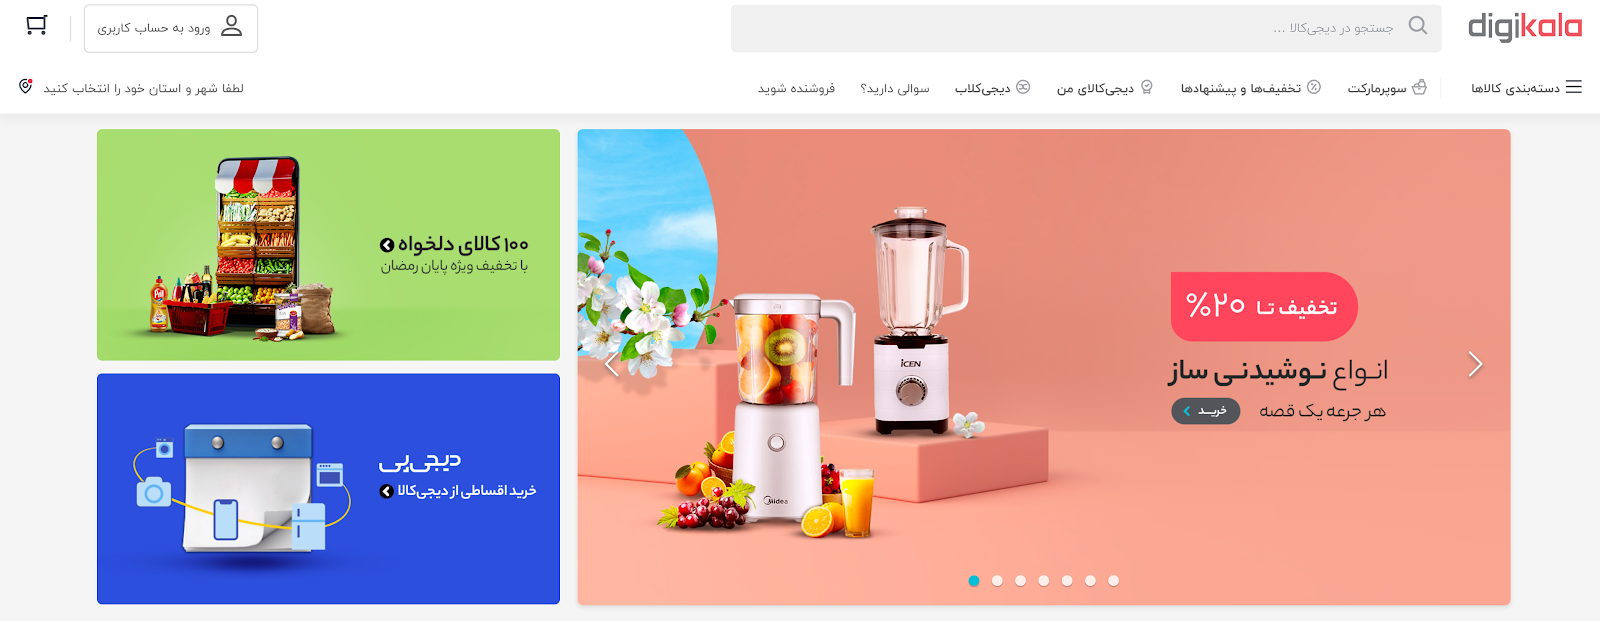
\includegraphics[width=0.9\textwidth]{images/image34.png}
\end{center}

\subsection*{{\titr انیمیشن در اسلاید   }}
\addcontentsline{toc}{subsection}{{\fehrestContent انیمیشن در اسلاید  }}


اسلاید‌های  شما می‌تواند همراه انیمیشن باشد. (یعنی ورود اسلاید و خروج آن انیمیشن داشته باشد)
 
 
\subsection*{{\titr ویدیو  }}
\addcontentsline{toc}{subsection}{{\fehrestContent ویدیو  }}


می‌توانید برای هر محصول در صفحه آن، علاوه بر عکس قابلیت قرار دادن ویدیو قرار دهید.


\subsection*{{\titr اسکرول  }}
\addcontentsline{toc}{subsection}{{\fehrestContent اسکرول  }}

قابلیت scroll در صفحاتی که لیست (لیست محصولات و لاگ‌ها و ...) نمایش داده می‌شود وجود داشته باشد.


\newpage

\subsection*{{\titr صفحه بندی  }}
\addcontentsline{toc}{subsection}{{\fehrestContent صفحه بندی  }}


در صفحاتی که لیستی از محصولات نمایش داده می‌شود (صفحه محصولات و حراج‌ها) در صورتی که مثلا تعداد محصولات از ۲۰ تا بیشتر باشد، مابقی را به صفحات بعدی منتقل کند، و در پایین لیست، قابلیت انتخاب شماره صفحه وجود داشته باشد.


 \begin{center}
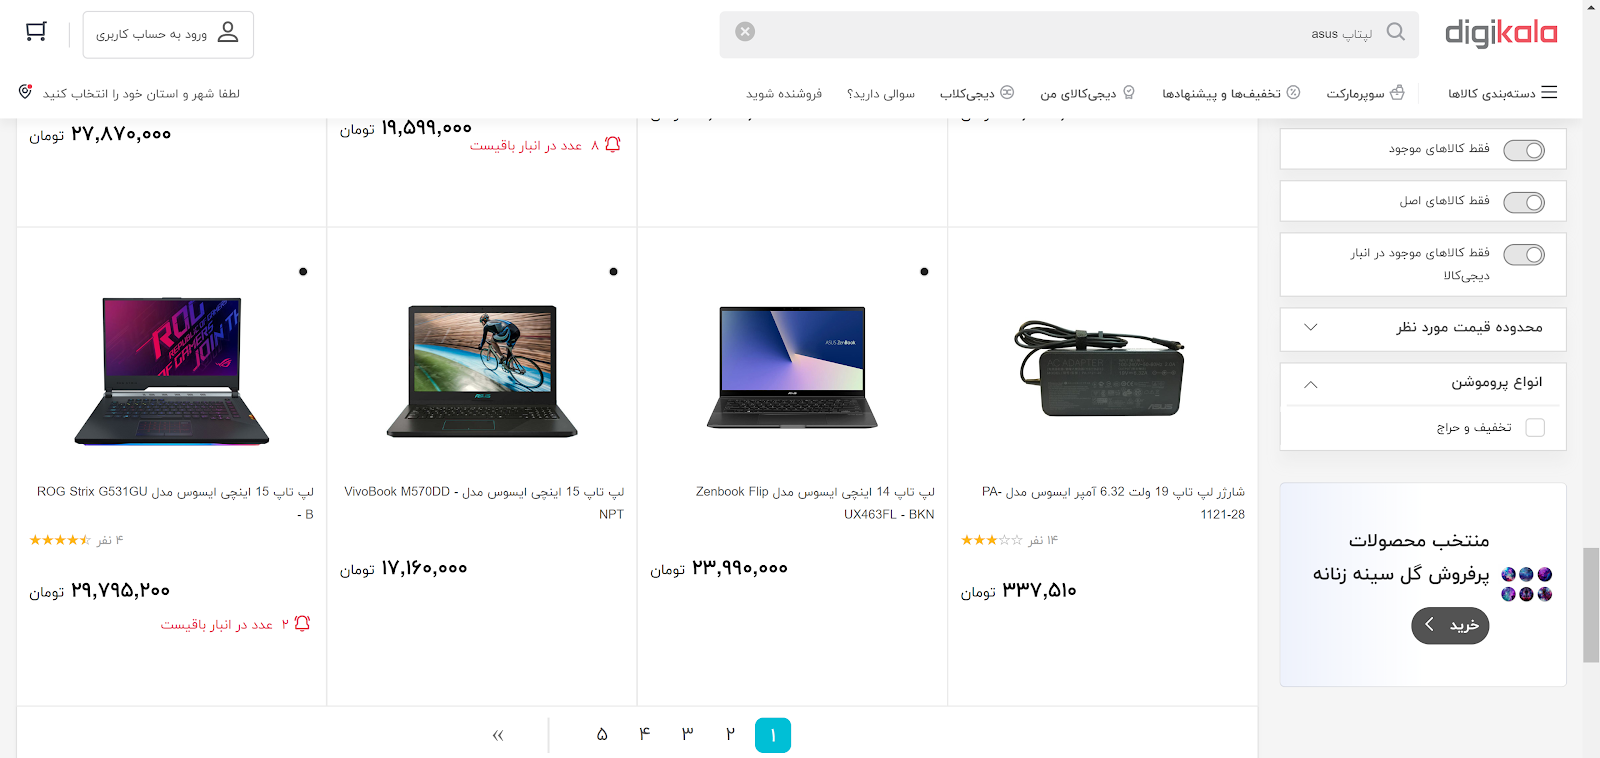
\includegraphics[width=0.9\textwidth]{images/image35.png}
\end{center}


\section*{{\titr لینک‌های آموزشی }}
\addcontentsline{toc}{section}{{\fehrestContent لینک‌های آموزشی }}

\begin{itemize}

\item
\href{https://www.javatpoint.com/javafx-tutorial}{\textcolor{blue}{\underline{\lr{java point}}}}

\item
\href{https://www.tutorialspoint.com/javafx/index.htm}{\textcolor{blue}{\underline{\lr{tutorials point}}}}

\end{itemize}




\end{document}







